% !TEX root=exama-220907.tex
%--------------------------------------
% Create title frame
\titleframe

%--------------------------------------
% Table of contents
\begin{frame}{Overview}
  \setbeamertemplate{section in toc}[sections numbered]
  \tableofcontents[hideallsubsections]
\end{frame}


%==============================================
\section{Introduction}
%==============================================
\begin{frame}{\insertsectionhead}
  \framesubtitle{ExaMA}
  NUMPEX/ExaMa concentrates on the exascale aspects of the numerical methods, ensuring their scalability to existing and forthcoming hardware.
  \vfill
  Leaders: C Prud'homme \& H Barucq
  \begin{itemize}
    \item 5 Work packages, may be spit even more
    \item wide range of topics: 
    \begin{itemize}
        \item Modeling and discretize
        \item  Linear, multi-linear and coupled solvers at Exascale
        \item Combine data and  models at Exascale
        \item Optimize and quantify uncertainties at Exascale
    \end{itemize}
    \item Demonstrators through mini-apps will be used to verify the properties of the methods and algorithms developed.
    
  \end{itemize}
\end{frame}
\begin{frame}{\insertsectionhead}
    
   \begin{itemize}
    \item 10 persons in initial work groups
    \item other teams consulted on various topics 
    \item 7 Mio Euros budget
\end{itemize} 
\end{frame}

\begin{frame}[fragile=singleslide]{\insertsectionhead}
  \framesubtitle{\insertsubsectionhead}
  \scriptsize
  \begin{columns}[]
    \begin{column}{.5\linewidth}
      \begin{itemize}
        \item (B1) Energy efficiency
        \item (B2) Interconnect Technology
        \item (B3) Memory technology
        \item (B4) Scalable systems software
        \item (B5) Programming systems
        \item (B6) Data Management
        \item (B7) Exascale Algorithms
      \end{itemize}
    \end{column}
    \begin{column}{.5\linewidth}
      \begin{itemize}
        \item (B8) Discovery, design, and decision algorithms
        \item (B9) Resilience, robustness and accuracy
        \item (B10) Scientific productivity
        \item (B11) Reproducibility, replicability of computation
        \item (B12) Pre/Post-processing
        \item (B13) Integrate Uncertainties
      \end{itemize}
    \end{column}
  \end{columns}

  
\end{frame}
%==============================================
\section{Status, milestones and Budget}
%==============================================

\subsection{Status}

\begin{frame}[fragile=singleslide]{\insertsectionhead}
  \framesubtitle{\insertsubsectionhead}
  \begin{itemize}
      \item Build WP team
      \item try to get people from CEA,INRIA,CNRS and University
      \item try to have both men and women in the steering team
      \item 2/3 co-lead per WP in charge of specific topics
      \item Some WPs will be probably further split
  \end{itemize}
  \begin{table}[]
      \centering
      \begin{tabular}{c|c}
          WP1 &  S Lanteri, V Faucher C Prud'homme H Barucq\\
          WP2&  L Grigori, L Giraud ...\\
          WP3& E Blayo, M Nodet, M Asch \\
          WP4& C Prieur, Cambodo? V Monbet, Y Privat, M Darbas, H Barucq \\
          WP5 & CEA/DAM? C Prud'homme
      \end{tabular}
      \caption{WP}
      \label{tab:my_label}
  \end{table}

\end{frame}

\subsection{Core Sites}

\begin{frame}[fragile=singleslide]{\insertsectionhead}
  \framesubtitle{\insertsubsectionhead}
  \begin{table}[H]
    \centering
    \caption{Core sites (to be discussed)}
    \begin{tabular}{@{} ccc @{}}
      \toprule
      \textbf{CEA} & \textbf{University/CNRS}  & \textbf{INRIA} \\
      \midrule
      CEA-DAM & Sorbonne Universités  & Inria Paris\\
      CEA-DES &  Université de Strasbourg &  Inria Bordeaux\\
      CEA-DRF & Université de Pau/Toulouse & Inria Sofia\\
      & Université Grenoble Alpes & Inria Lyon\\
      & Université Paris Saclay	& Inria Lille \\
      \bottomrule
    \end{tabular}
  \end{table}

\end{frame}
\begin{frame}[fragile=singleslide]{\insertsectionhead}
  \framesubtitle{\insertsubsectionhead}
  
  Some issues/questions:
  \begin{itemize}
      \item potentially a lot of teams interested, find the right level
      \item any policies about leaders  involvement  and their team?
  \end{itemize}
  
\end{frame}
%--------------------------------------
\subsection{Expected results}

\begin{frame}
  \frametitle{\insertsectionhead}
  \framesubtitle{\insertsubsectionhead}
  \begin{itemize}
      \item   Methods, algorithms, and implementations that, taking advantage of the exascale architectures, empower modeling, solving, assimilating model and data, optimizing and quantifying uncertainty, at levels that are unreachable at present.
    \item Software libraries allowing to assemble specific critical reusable components, hiding the hardware complexity and exposing only the specific methodological interface
    \item Methodological and Algorithmic Patterns at exascale that can be reused efficiently in large scale applications (eg in weather forecasting)
    \item Enabling AI algorithms to attain performances at exascale, exploiting the methods (point 1) and the libraries (point 2) developed.
    \item \href{https://docs.google.com/document/d/1hjwSFRF63SyTUJJKGMNLHcJPr_S2JDHYXeBeQzHCSno/edit?usp=sharing}{\beamergotobutton{Demonstrators}}

  \end{itemize}


\end{frame}

\subsection{Milestones}

\begin{frame}
  \frametitle{\insertsectionhead}
  \framesubtitle{\insertsubsectionhead}
  \begin{itemize}
      \item   M1 Select IP-1 use-cases/demonstrators and associate methodology developments T0+6
\item M2 benchmark IP-1 demonstrators on pre-exascale systems T0+9/T0+12
\item M3 enable and benchmarks some new exascale  IP-1 components on pre-exascale/exascale systems T0+18, T0+36, T0+54, T0+60
  \end{itemize}


\end{frame}

\subsection{Budget}

\begin{frame}
  \frametitle{\insertsectionhead}
  \framesubtitle{\insertsubsectionhead}

  \begin{itemize}
    \item large project involved many teams
    \item need enough momemtum
    \item initially 7Mio Euro
    \item proposed budget 6Mio Euro
    \item 
  \end{itemize}

\end{frame}
%==============================================
\section{Relations}
%==============================================
\subsection{Industry}
\begin{frame}{\insertsectionhead}
  \framesubtitle{\insertsubsectionhead}
Contacted Entreprises
\begin{itemize}
    \item EdF
    \item Safran
\end{itemize}
To be contacted
\begin{itemize}
    \item Arkema
    \item Total
    \item PlasticOmnium
    \item Atos
    \item Entreprises from Consortium Mordicus
    \item ...
\end{itemize}
\end{frame}

\subsection{PEPR}
\begin{frame}{\insertsectionhead}
  \framesubtitle{\insertsubsectionhead}

\begin{itemize}
    \item IA
    \item Diadem ?
    \item TRACCS-Météo?
\end{itemize}

Links were made with CMA IA MAIAGE (training), results end of September.
\end{frame}

\subsection{Europe}
\begin{frame}{\insertsectionhead}
  \framesubtitle{\insertsubsectionhead}
\begin{itemize}
    \item Coe Hidalgo-2 
    \item ERC-Synergy	EMC2
    \item EuroHPC	Microcard
    \item H2020 RIA Digital Twin	Bim2Twin
    \item CoE	EoCoE-3	
    \item EuroHPC	European Master for HPC - EUMaster4HPC	
\end{itemize}
\end{frame}

\subsection{Interactions with Genci and Tier-0}
\begin{frame}{\insertsectionhead}
  \framesubtitle{\insertsubsectionhead}

\begin{itemize}
    \item TBD
\end{itemize}
\end{frame}

\section{GitHub}
\subsection{Project planning}
\begin{frame}
  \frametitle{\insertsectionhead}
  \framesubtitle{\insertsubsectionhead}
  \begin{itemize}
      \item Create issues(tasks), 
      \item break them into tasks, 
      \item track relationships, 
      \item add/use custom fields, 
      \item and have conversations. 
  \end{itemize}
  \alert{Visualize large projects as spreadsheets or boards, and automate everything with code.}
\end{frame}
\subsection{Table vs Board Views}
\begin{frame}
  \frametitle{\insertsectionhead}
  \framesubtitle{\insertsubsectionhead}
  \begin{columns}{T}
    \column{.45\textwidth}
    \begin{itemize}
        \item Built like a spreadsheet, project tables give a live workspace to filter, sort, and group issues and pull requests. 
        \item We can tailor them to your needs with custom fields and saved views.
        \item boards can display group issues using custom fields (e.g. Status)
    \end{itemize}
    \column{.5\textwidth}
    \only<1>{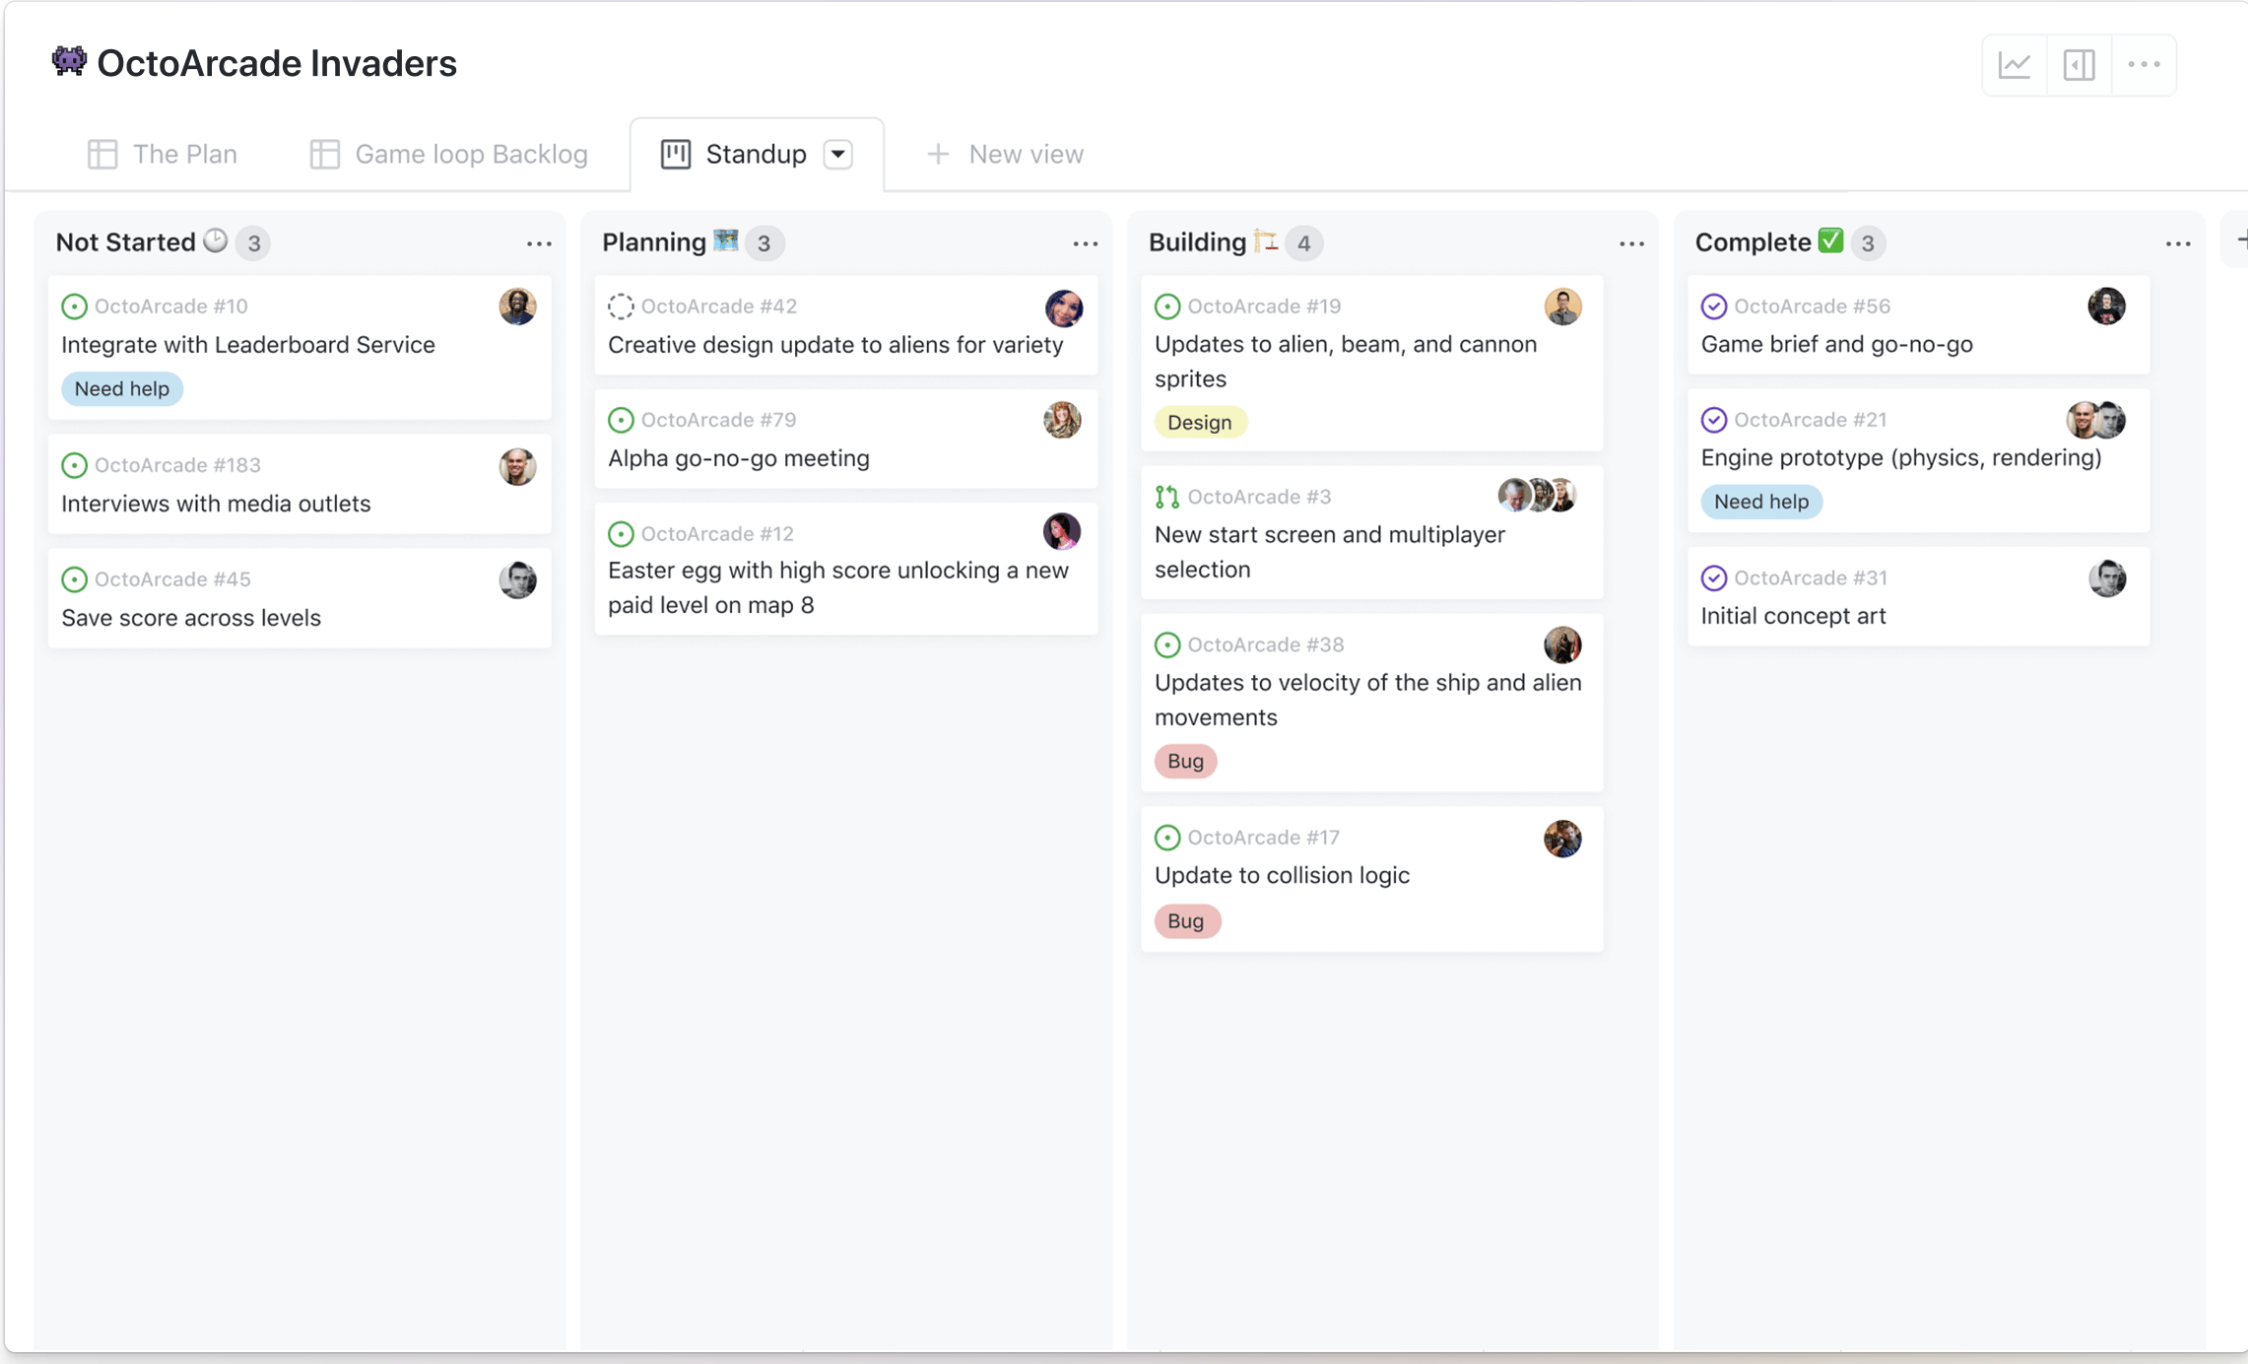
\includegraphics[width=.9\linewidth]{figures/board-view.png}}
    \only<2>{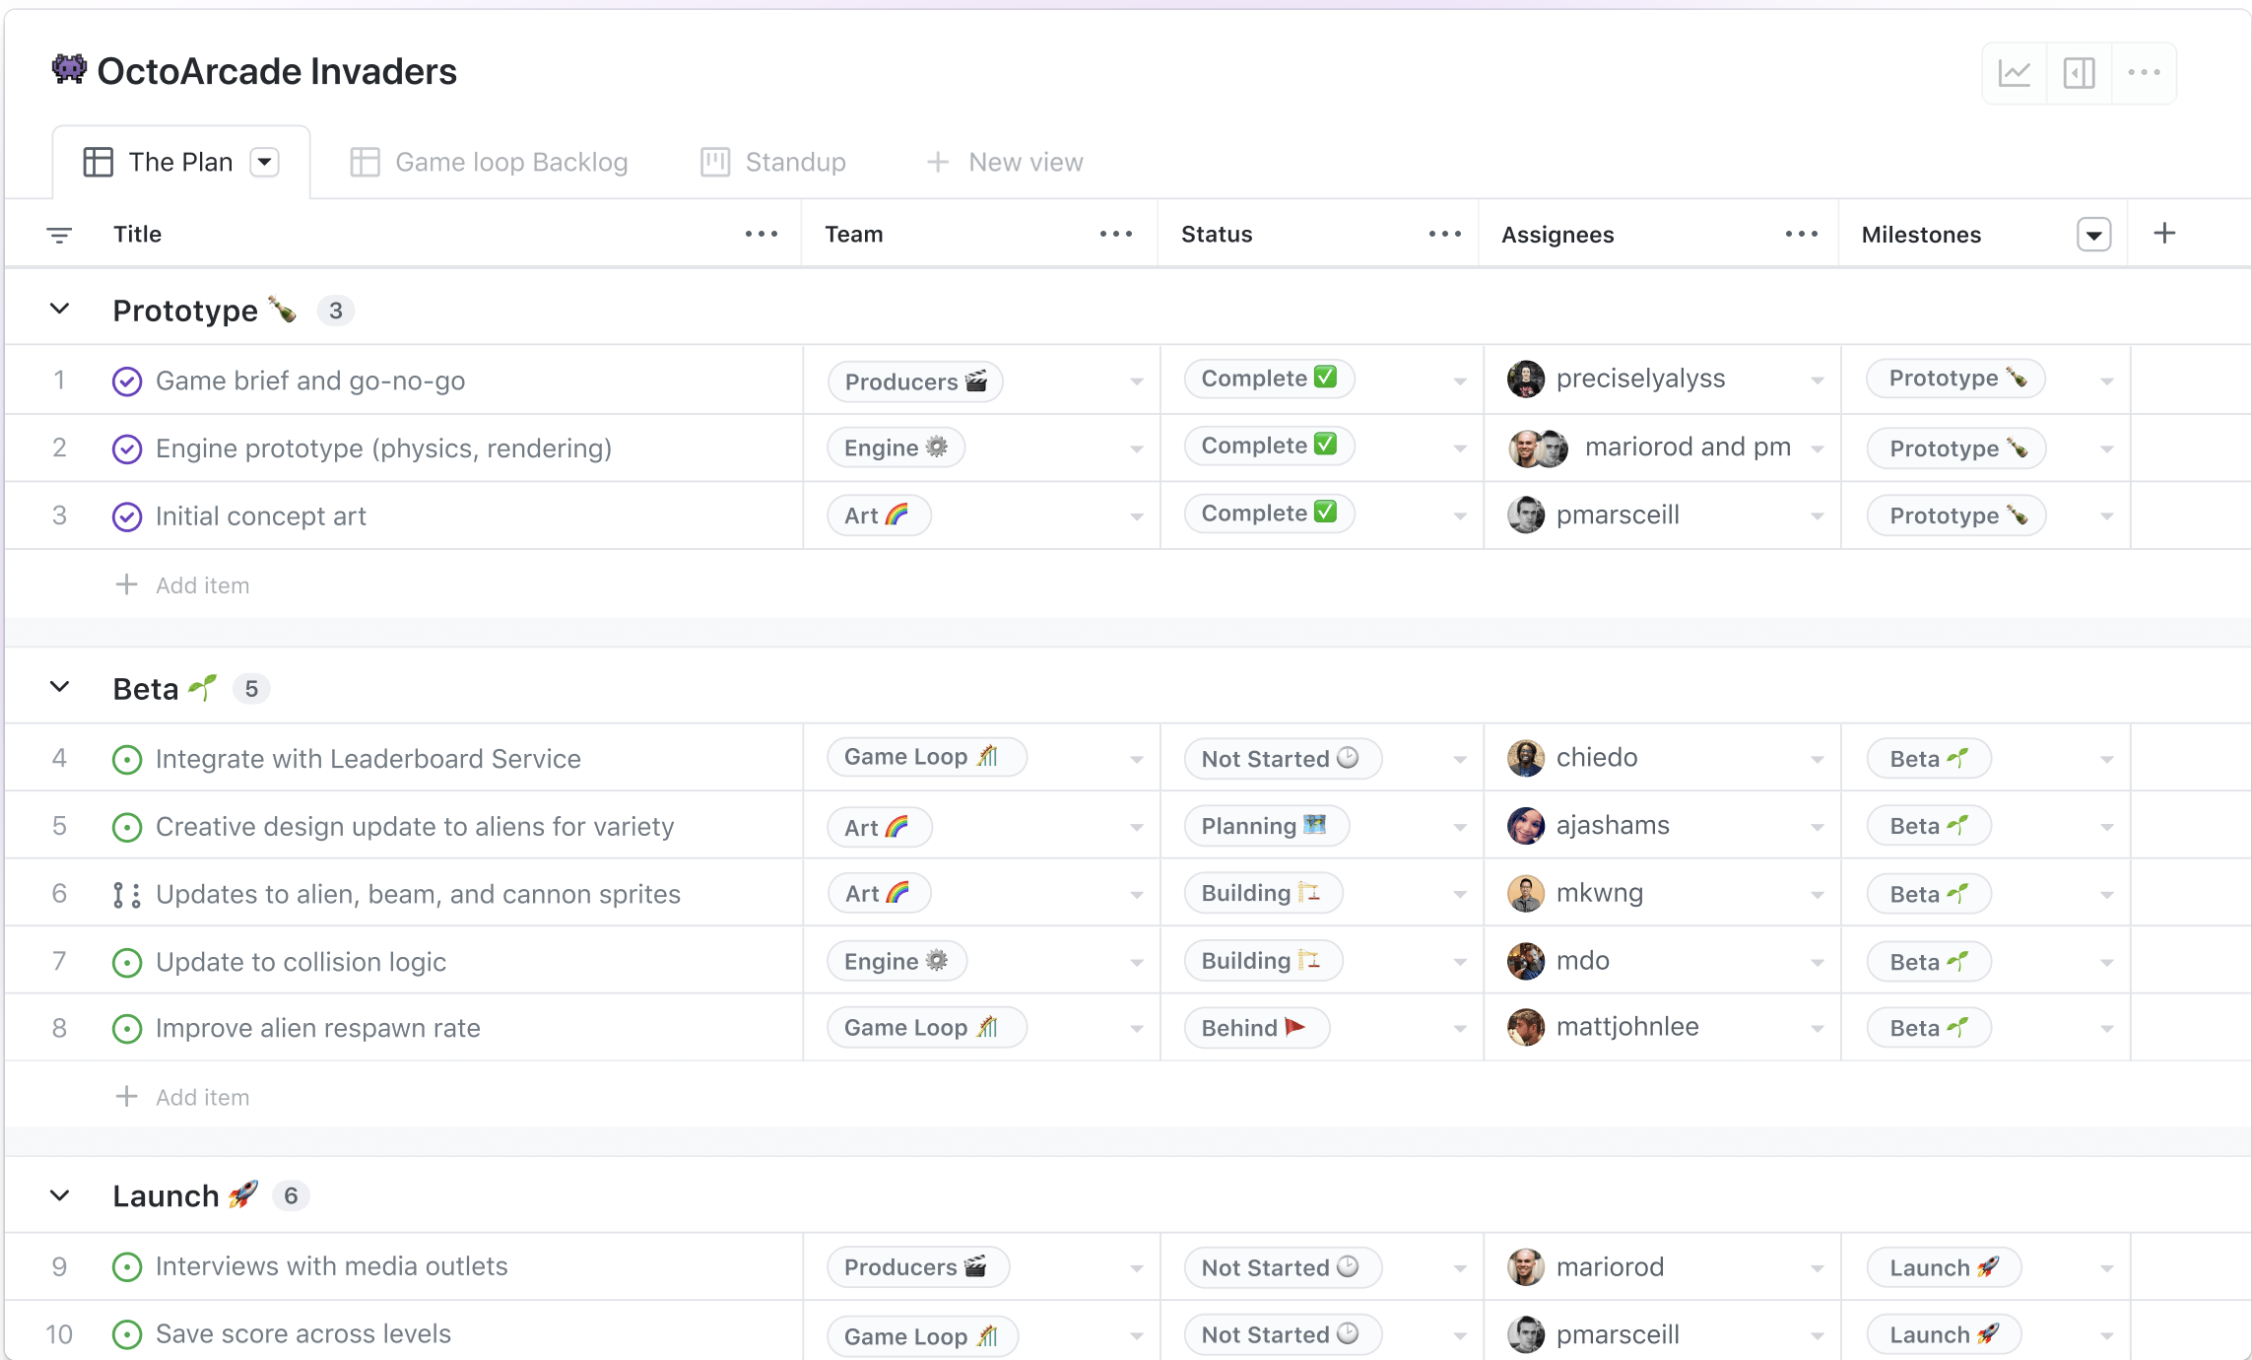
\includegraphics[width=.9\linewidth]{figures/table-view.png}}
  \end{columns}
\end{frame}

\subsection{Break issues into actionable tasks}

\begin{frame}
  \frametitle{\insertsectionhead}
  \framesubtitle{\insertsubsectionhead}
  \begin{columns}
    \column{.45\textwidth}
    \begin{itemize}
      \item Tackle complex issues with task lists 
      \item track their status with new progress indicators. 
      \item Convert tasks into their own issues 
      \item navigate your work hierarchy.
  \end{itemize}
  \column{.5\textwidth}
    \only<1>{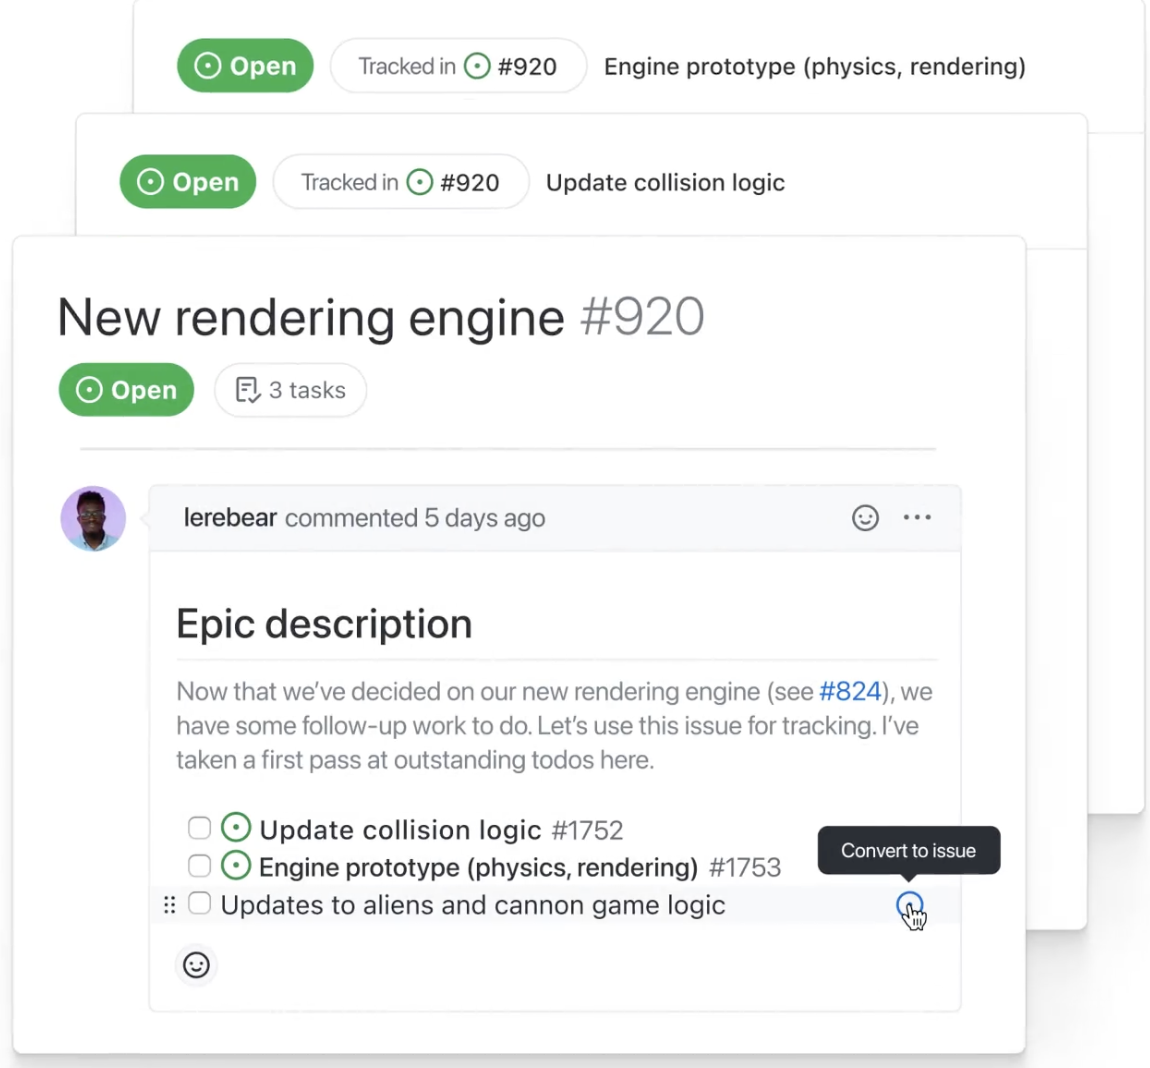
\includegraphics[width=.9\linewidth]{figures/issues-1.png}}
    \only<2>{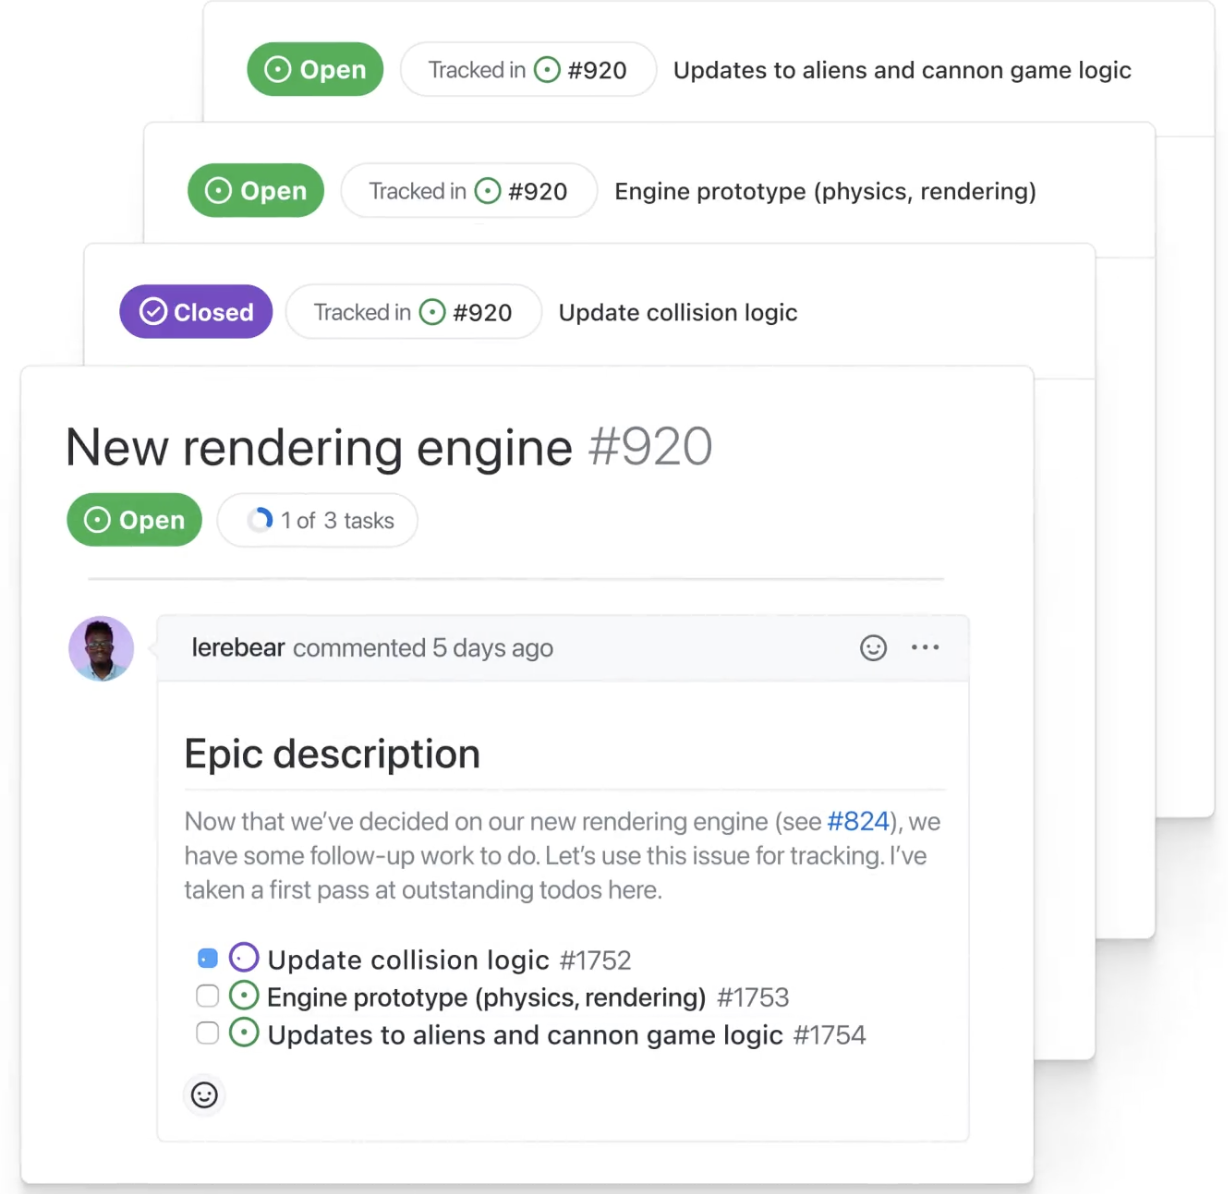
\includegraphics[width=.9\linewidth]{figures/issues-2.png}}
    \only<3>{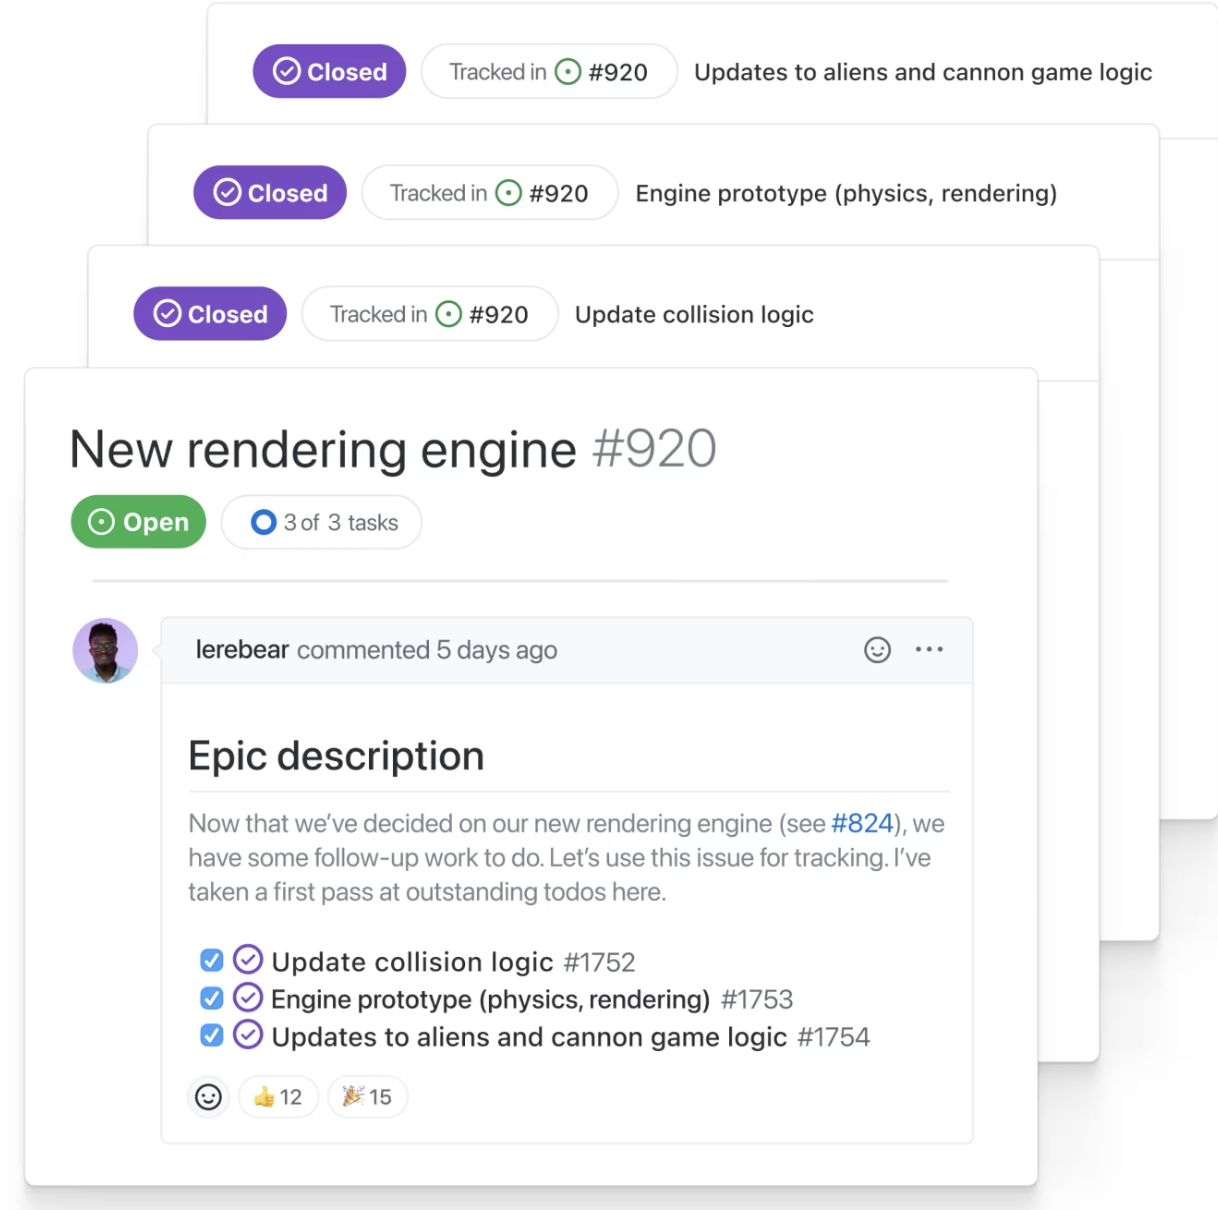
\includegraphics[width=.9\linewidth]{figures/issues-3.png}}
  \end{columns}
\end{frame}


\subsection{Conversations}

\begin{frame}
  \frametitle{\insertsectionhead}
  \framesubtitle{\insertsubsectionhead}
  \begin{columns}
    \column{.45\textwidth}
    \scriptsize
    \begin{itemize}
      \item Move conversations forward
      \item Express ideas with GitHub Flavored Markdown, 
      \item mention contributors, 
      \item react with emoji, 
      \item clarify with attachments(videos, pdf, images...), 
      \item see references from commits, pull requests, releases, and deploys. 
      \item Coordinate by assigning contributors and teams, 
      \item or by adding them to milestones and projects. 
    \end{itemize}
    \centering\vspace{1cm}
    \alert{All in a single timeline.}
    \column{.45\textwidth}
    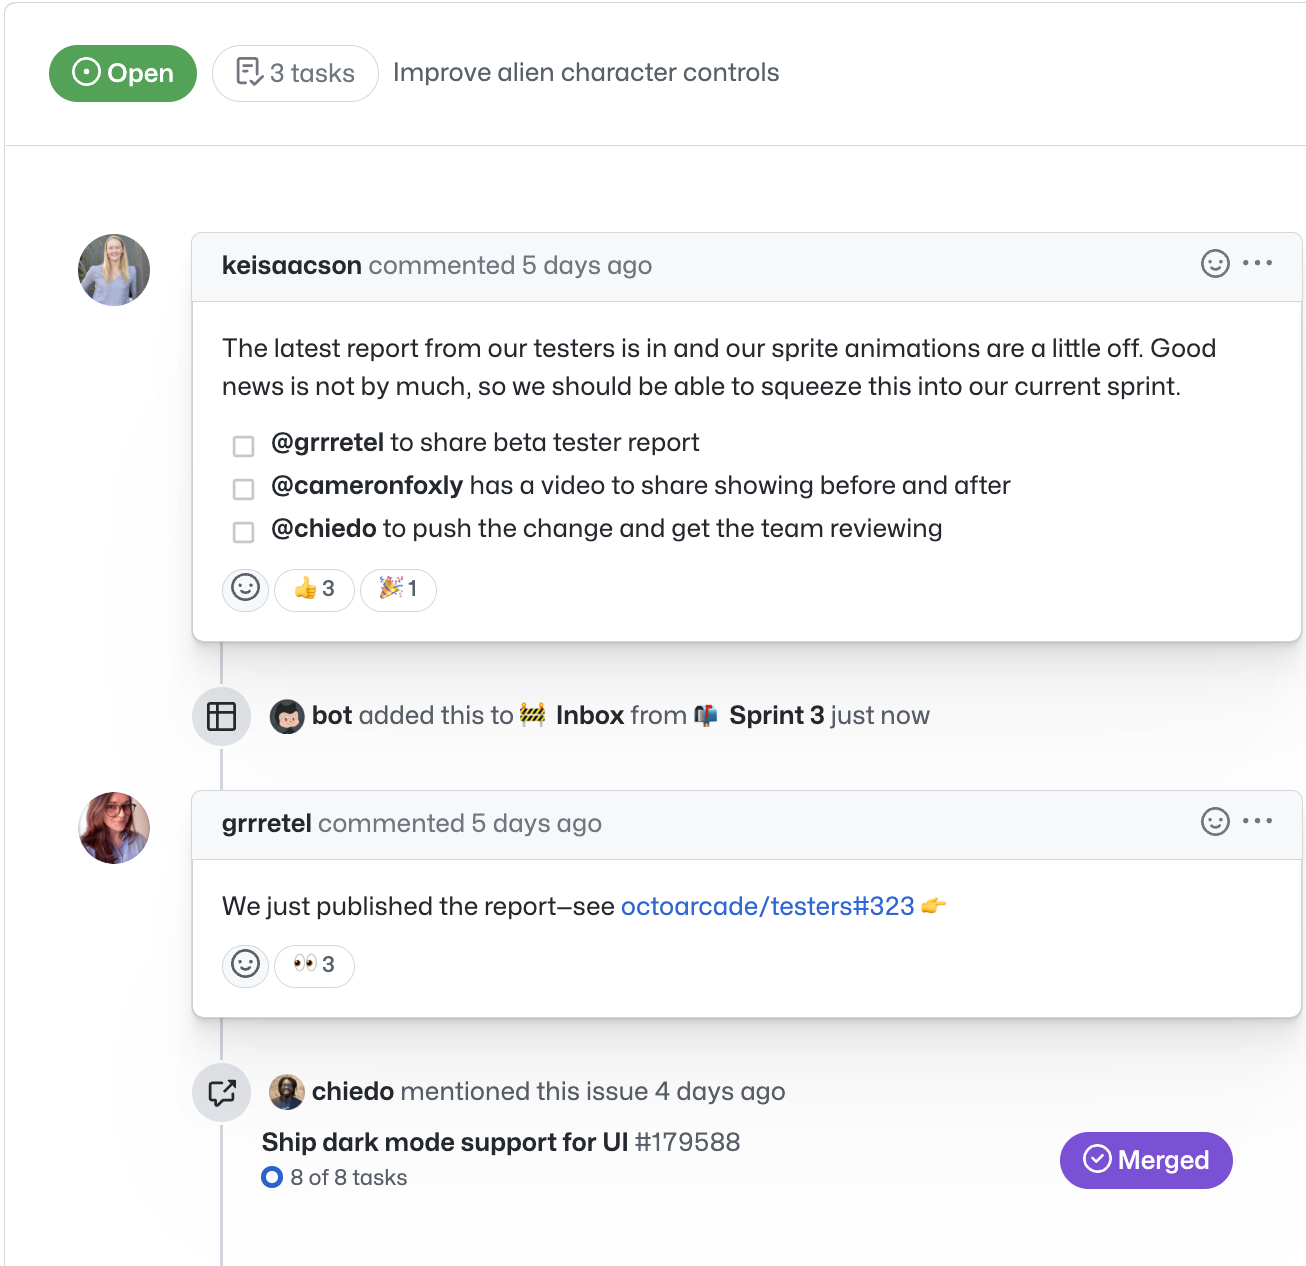
\includegraphics[width=.9\linewidth]{figures/conversations-1.png}
  \end{columns}

\end{frame}

\subsection{Create views}
\begin{frame}
  \frametitle{\insertsectionhead}
  \framesubtitle{\insertsubsectionhead}
  \begin{columns}
    \column{.4\textwidth}
    \begin{itemize}
      \item Save views for sprints, backlogs, teams, or releases. 
      \item Rank, group, sort, and filter issues to suit the occasion. 
      \item Choose between tables, boards, and timelines.
    \end{itemize}
    \column{.55\textwidth}
    \only<1>{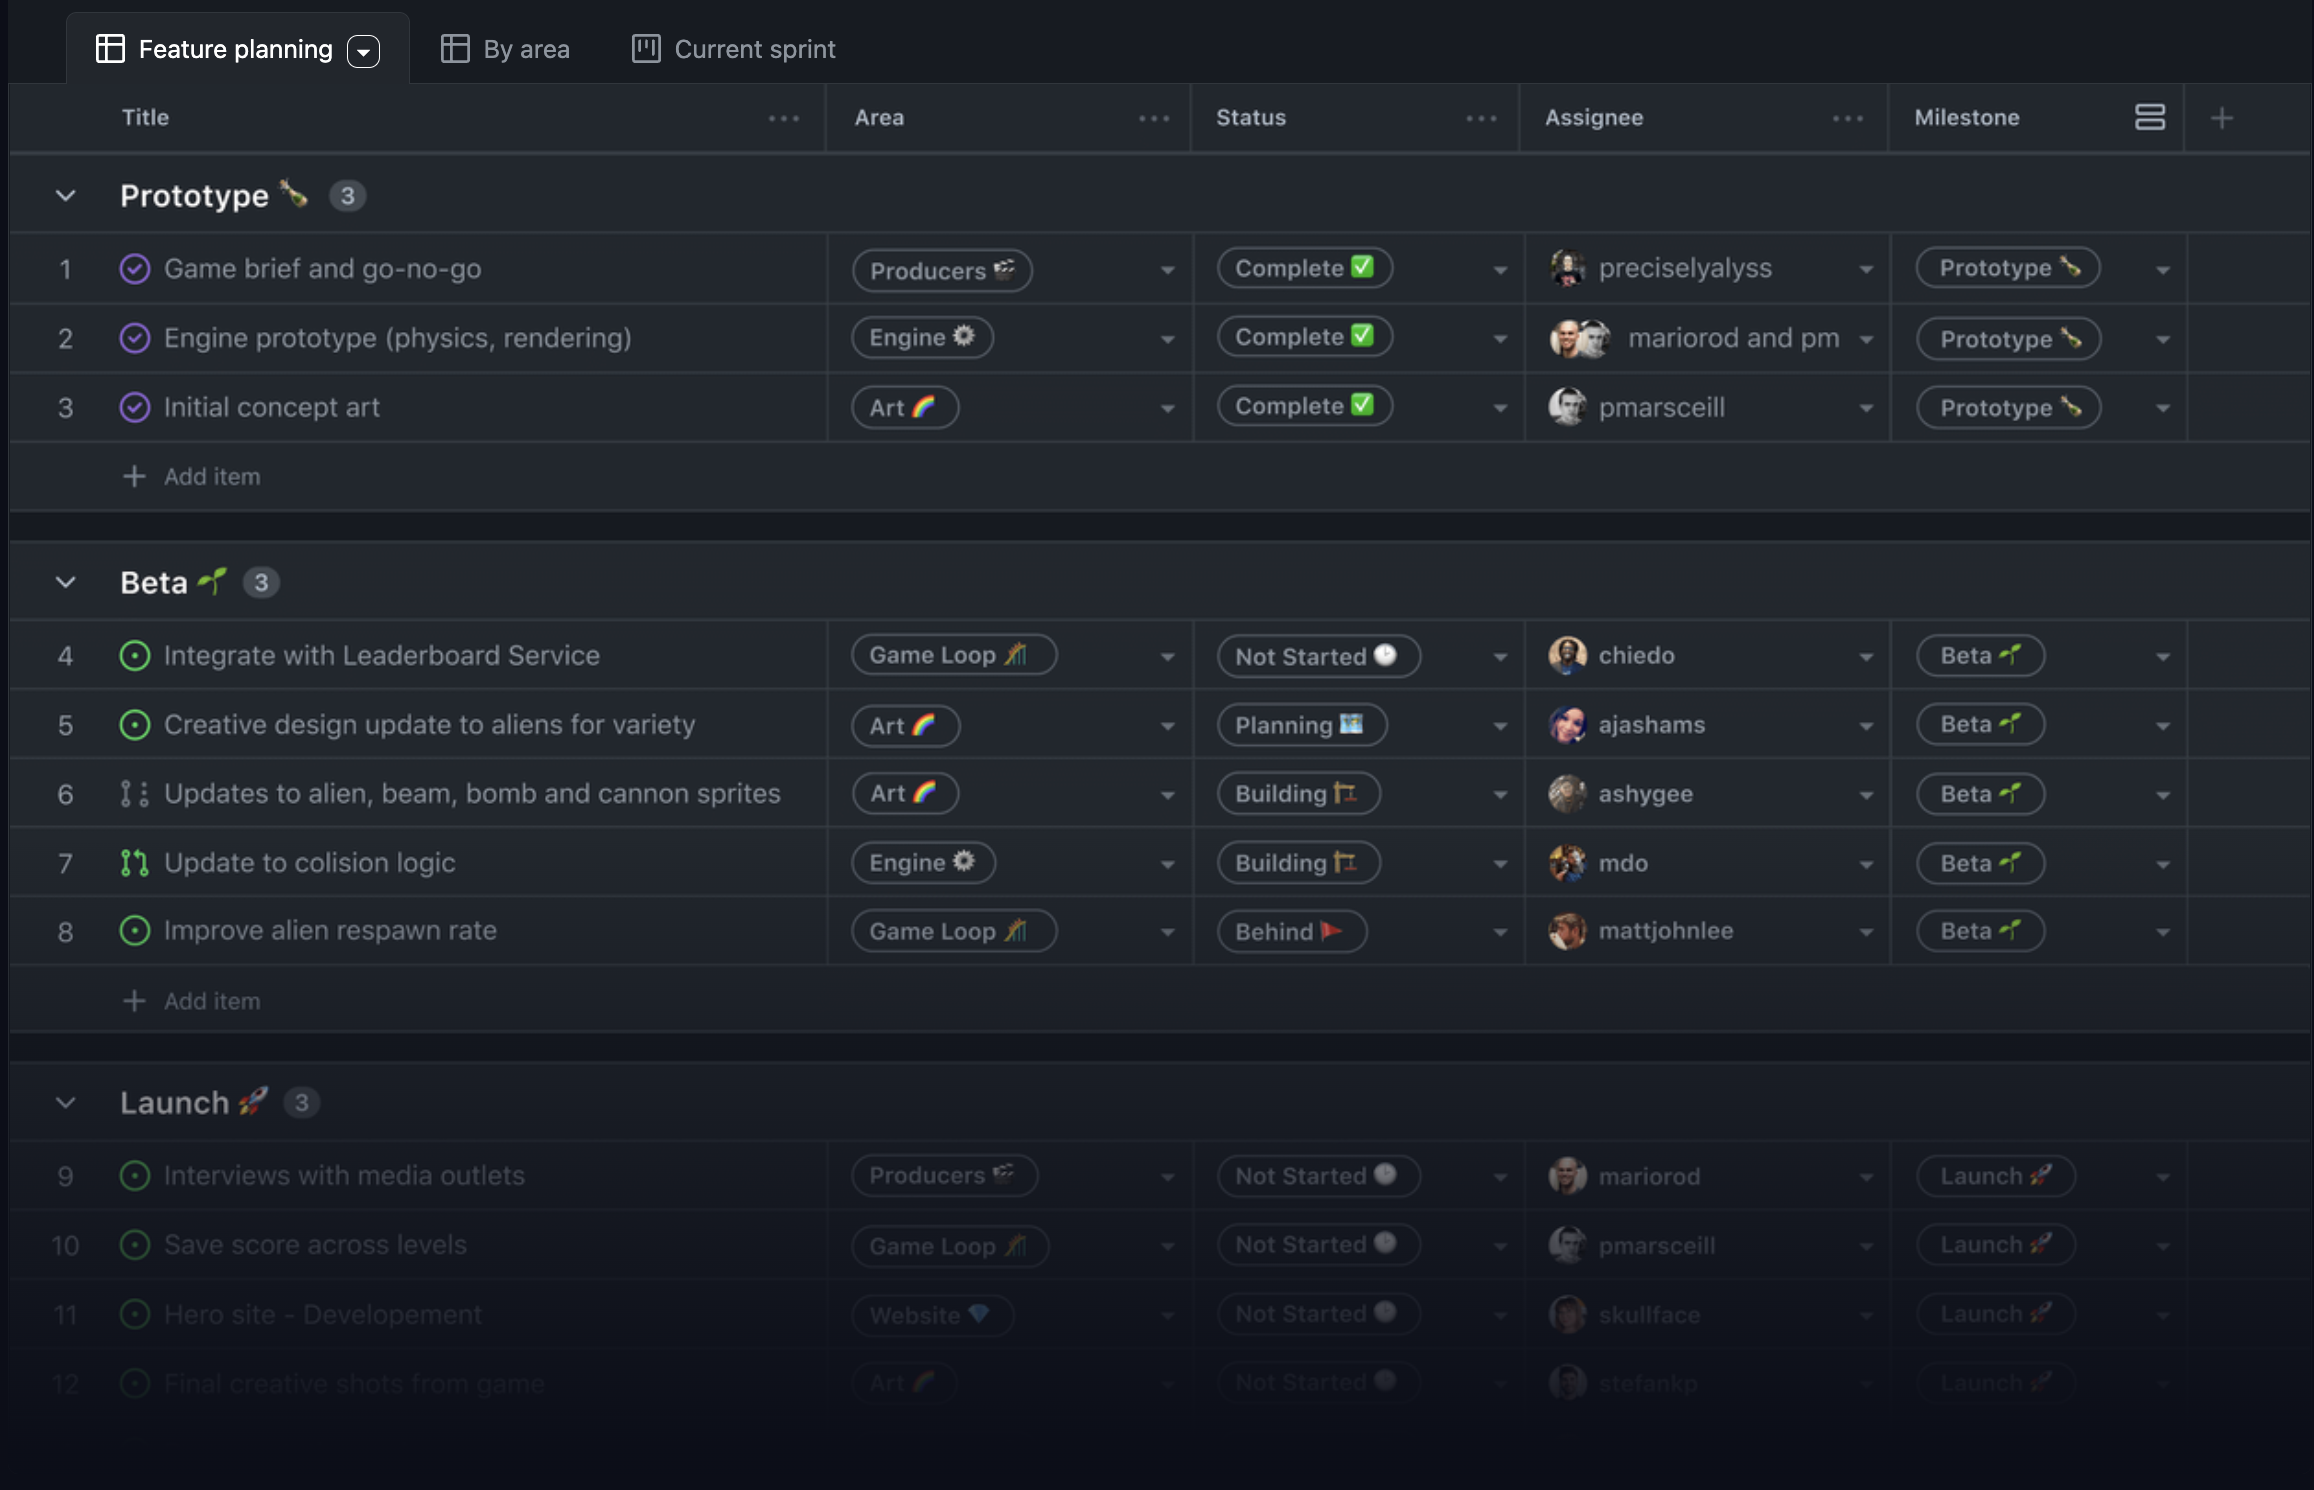
\includegraphics[width=.95\linewidth]{figures/views-1.png}}
    \only<2>{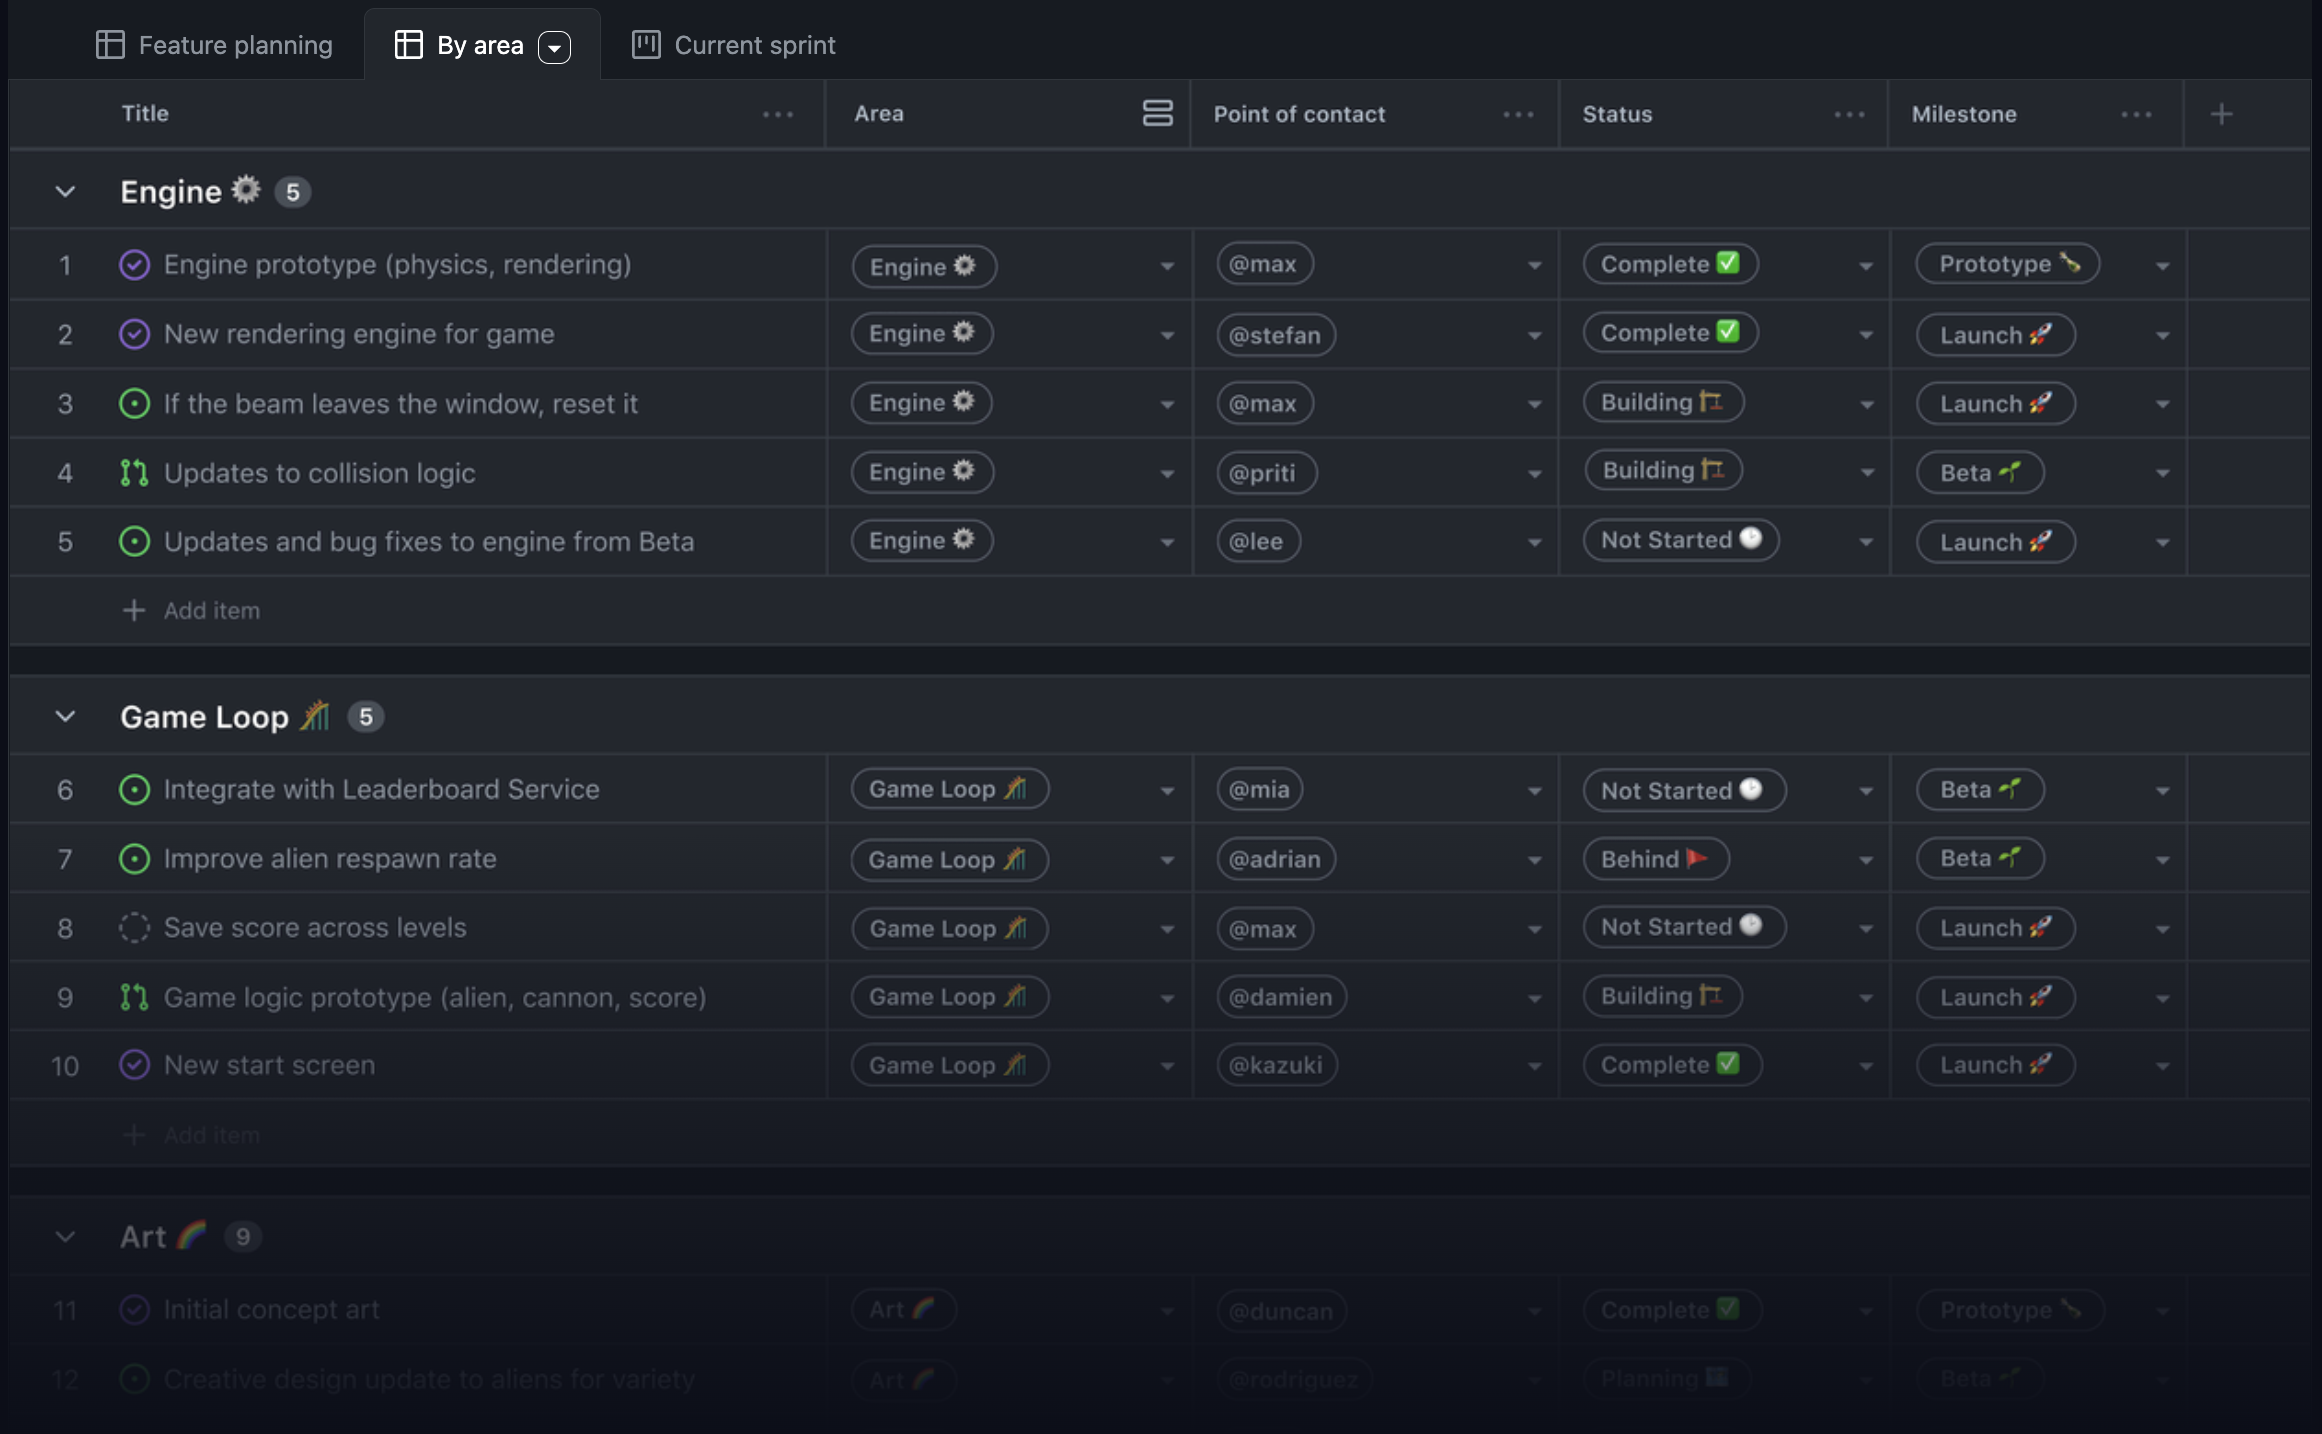
\includegraphics[width=.95\linewidth]{figures/views-2.png}}
    \only<3>{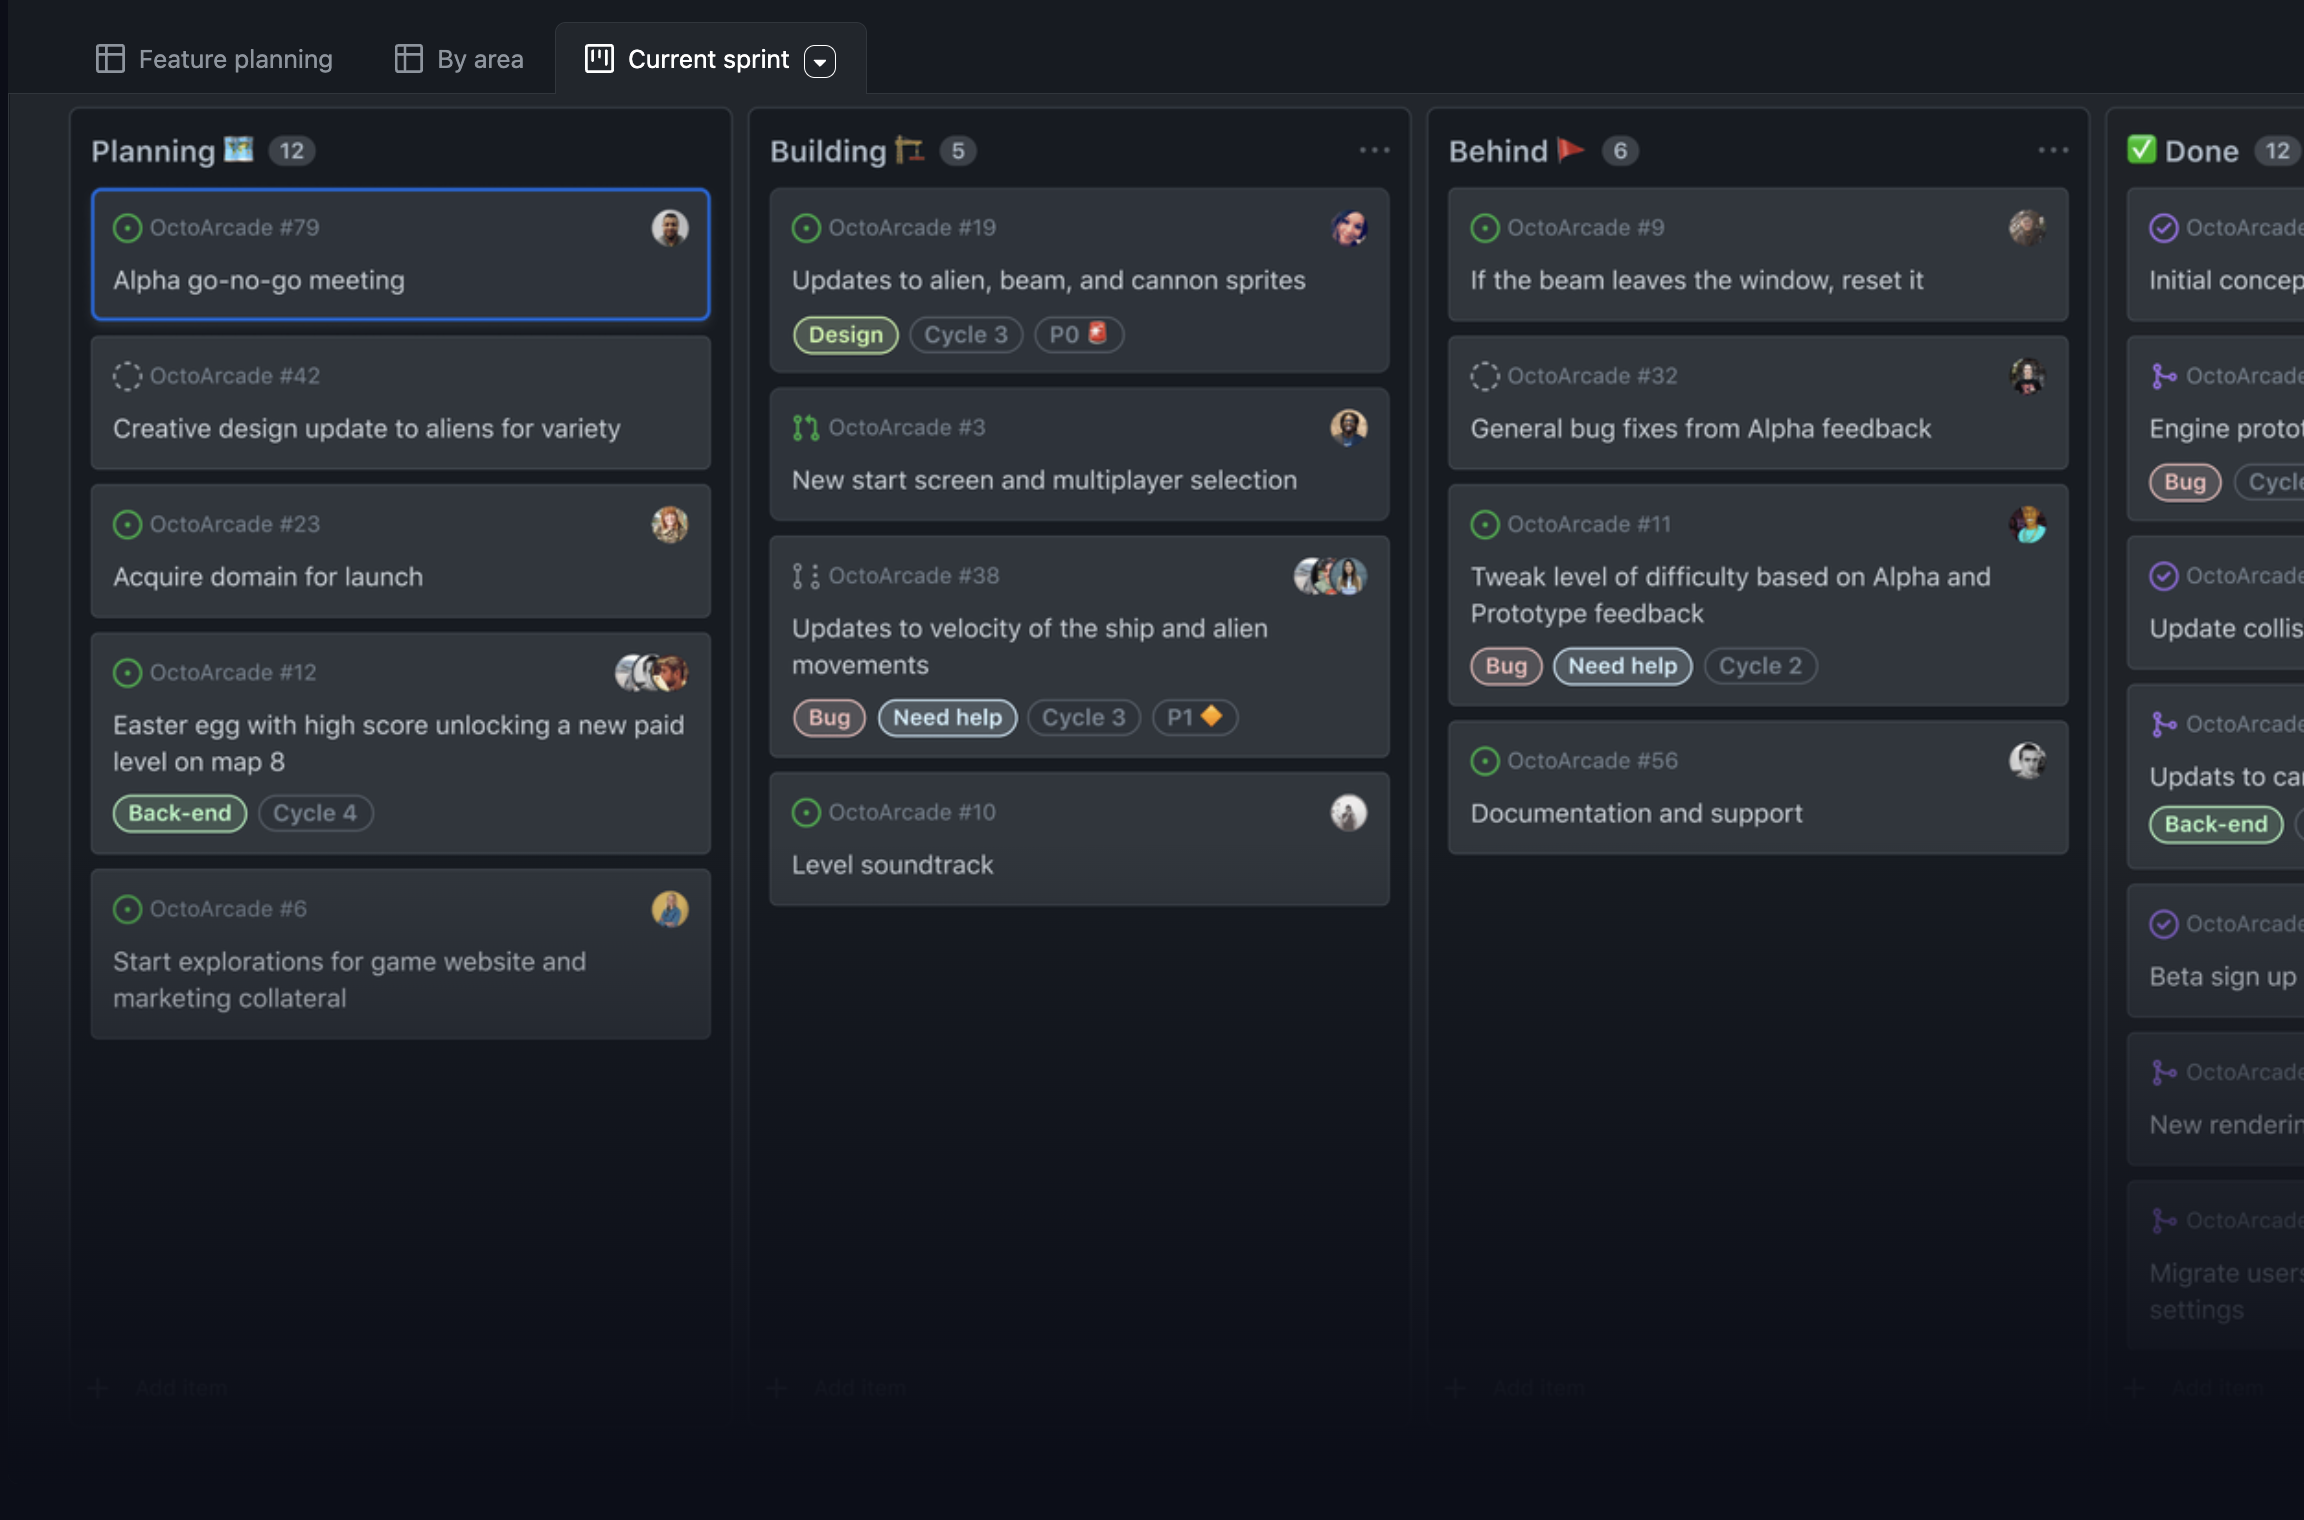
\includegraphics[width=.95\linewidth]{figures/views-3.png}}
  \end{columns}

\end{frame}

\subsection{Extend issues with custom fields}

\begin{frame}
  \frametitle{\insertsectionhead}
  \framesubtitle{\insertsubsectionhead}
  \begin{columns}
    \column{.4\textwidth}
    \begin{itemize}
      \item Track metadata like iterations, priority, story points, dates, notes, and links. 
      \item Add custom fields to project tables 
      \item edit from the issue sidebar.
    \end{itemize}
    \column{.55\textwidth}
    \only<1>{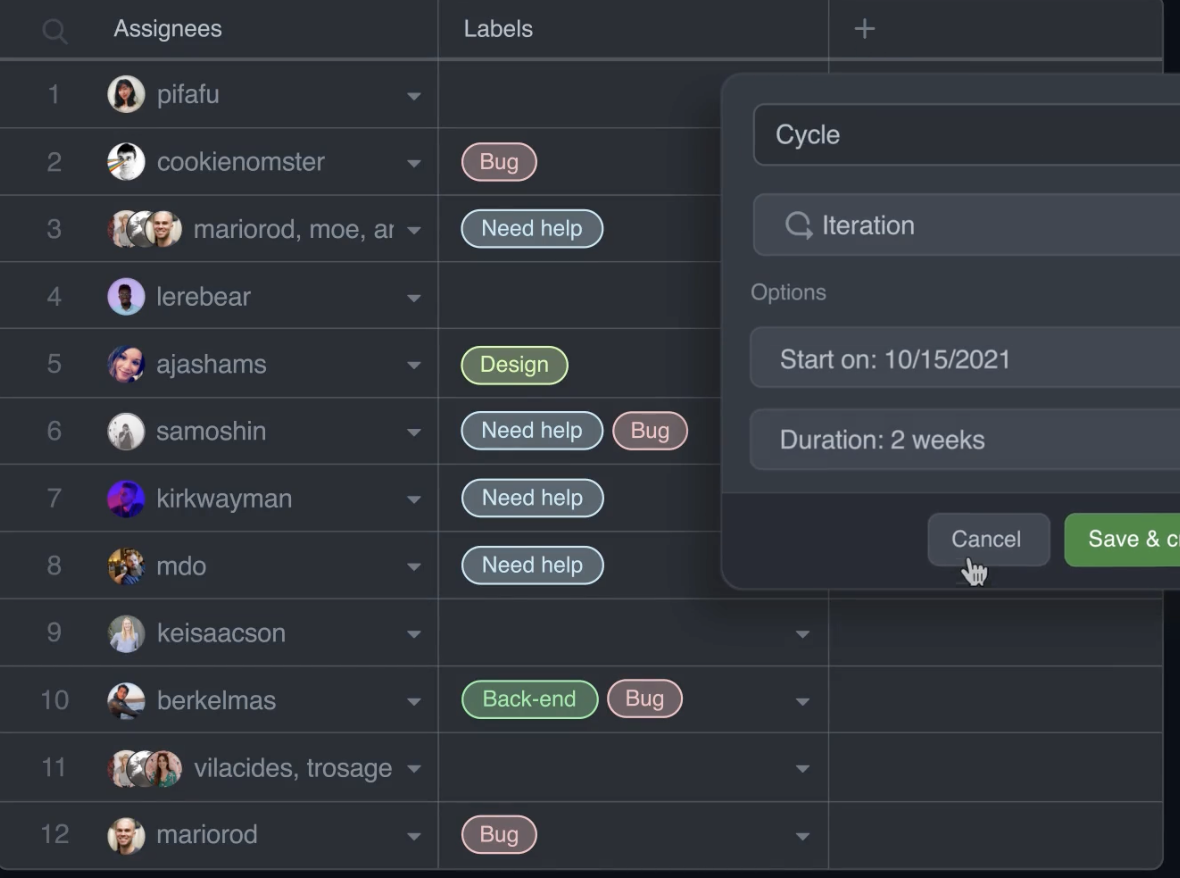
\includegraphics[width=.95\linewidth]{figures/custom-fields-1.png}}
    \only<2>{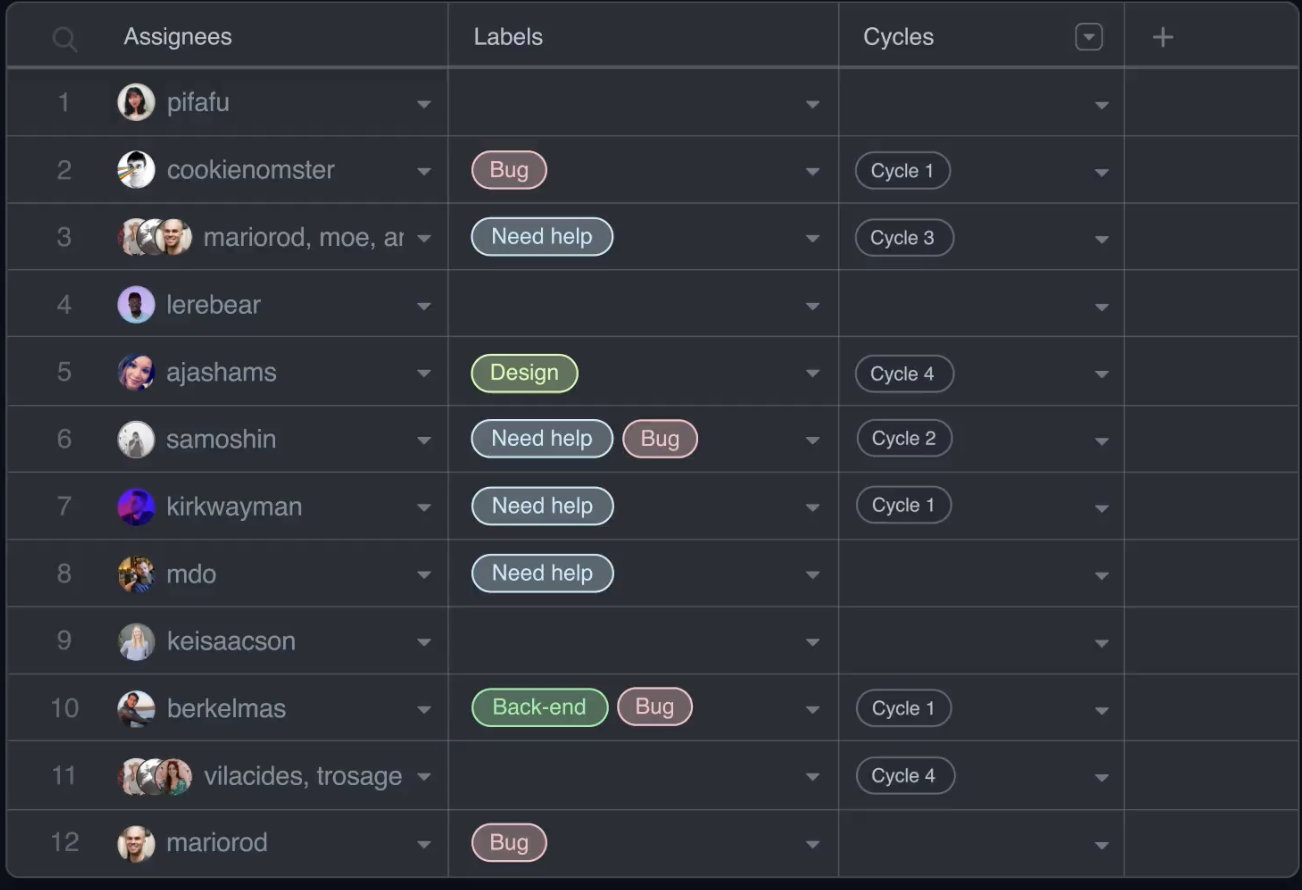
\includegraphics[width=.95\linewidth]{figures/custom-fields-2.png}}
  \end{columns}
  

\end{frame}
\begin{frame}
  \frametitle{\insertsectionhead}
  \framesubtitle{\insertsubsectionhead}

  \begin{columns}
    \column{.4\textwidth}
    \begin{itemize}
      \item Track the health of your current iteration cycle, milestone, or any other custom field you create with new project insights.
      \item  Identify bottlenecks and issues blocking the team from making progress with the burn up charts.
    \end{itemize}
    \column{.55\textwidth}
    \only<1>{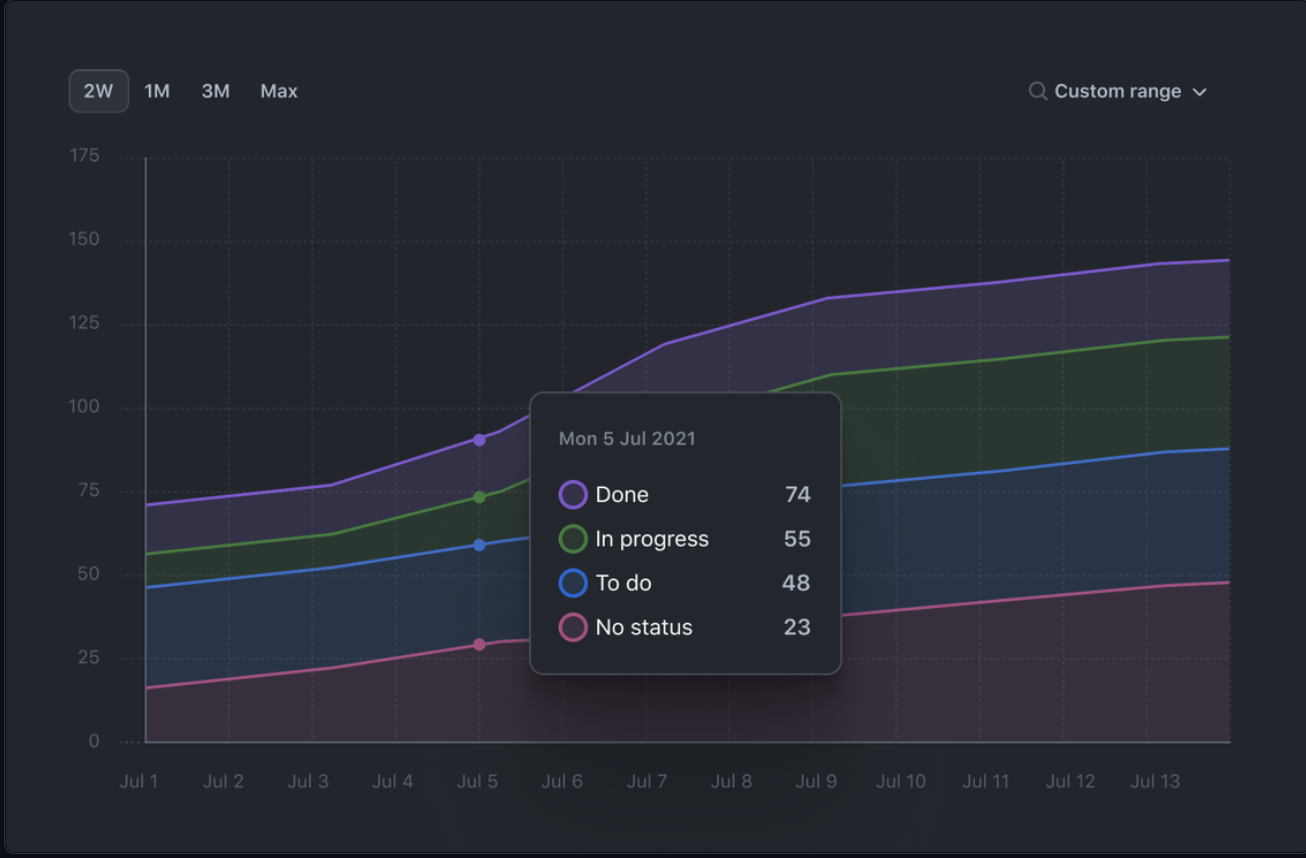
\includegraphics[width=.95\linewidth]{figures/charts-1.png}}
  \end{columns}


\end{frame}
\subsection*{Automate workflows}
\begin{frame}
  \frametitle{\insertsectionhead}
  \framesubtitle{\insertsubsectionhead}
  \begin{columns}
    \column{.4\textwidth}
    \begin{itemize}
      \item  Automate the project planning with workflows. 
      \item Automatically triage issues, set values for custom fields, react to changes, or schedule something. 
      \item You can even tee them up to run an Action.
    \end{itemize}
    \column{.55\textwidth}
    \only<1>{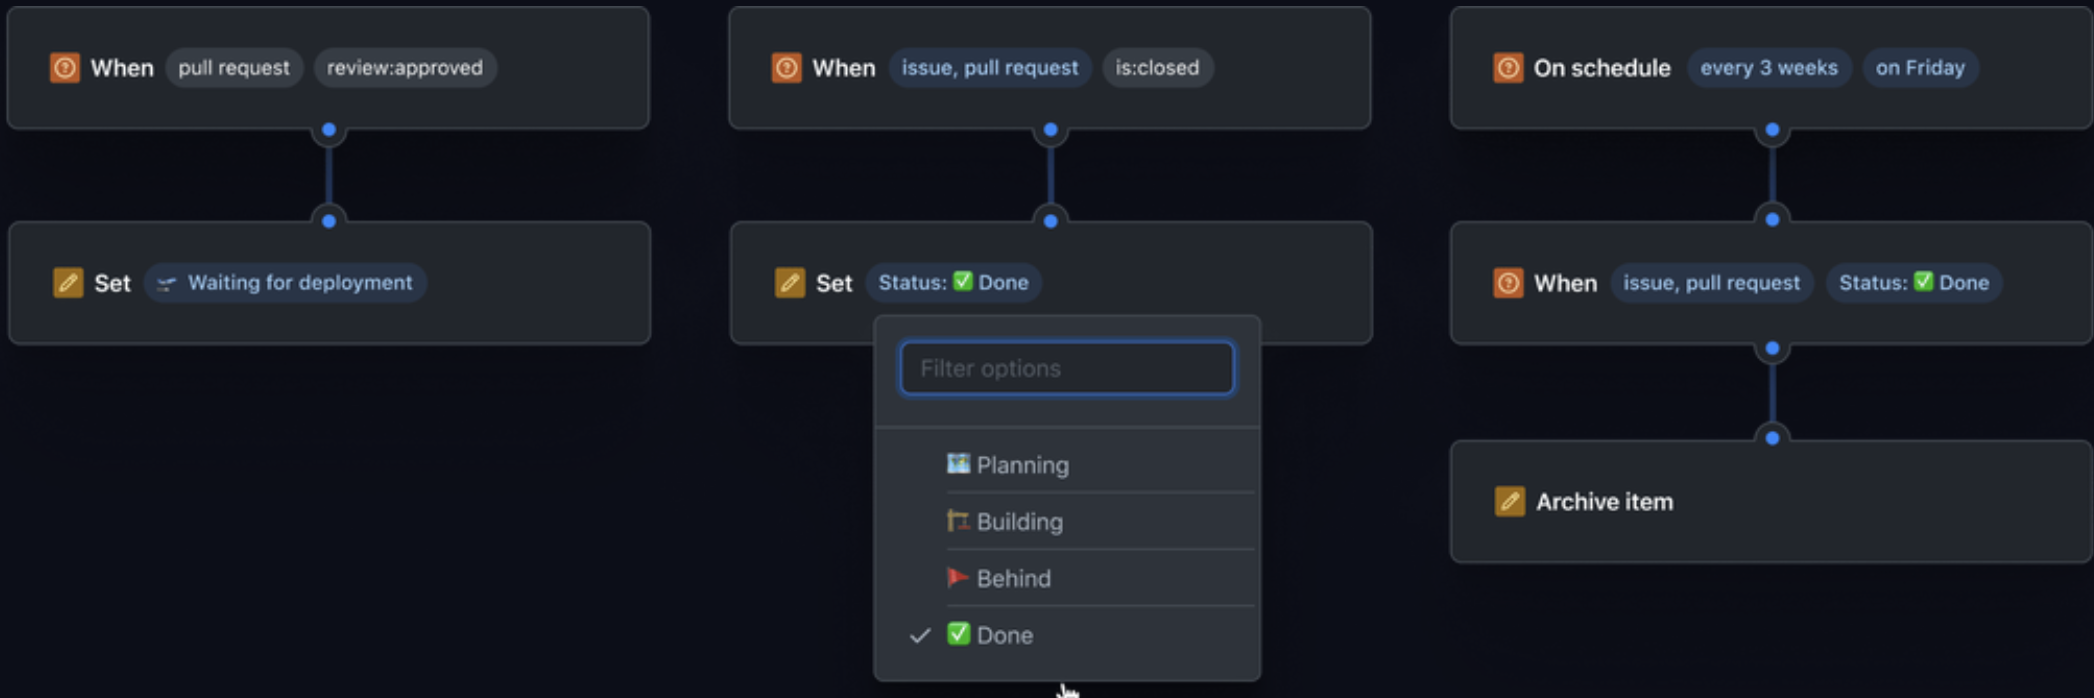
\includegraphics[width=.95\linewidth]{figures/workfflows-1.png}}
  \end{columns}

\end{frame}